\subsection{Omskrivning mellem ligheder og uligheder}
Da et programmeringsproblem ikke nødvendigvis er på den ønskede form fra start af, er det vigtigt at kunne omskrive mellem uligheder og ligheder.\\
\begin{itemize}
\item Omskrivning mellem uligheder %Det er blevet bedere, men er stadig ikke helt godt
\begin{align*}
	\vec{a}_i^T\vec{x} \geq b_i \quad \Leftrightarrow \quad -\vec{a}_i^T\vec{x} \leq -b_i
\end{align*}
\item Omskrivning fra lighed til ulighed % hvorfor bruges der forskellige pile. rettet
\begin{center}
\begin{tabular}{>{$}l<{$} >{$}r<{$}}
	\vec{a}_i^T\vec{x} = b_i \quad \Leftrightarrow \quad 	& 
	\vec{a}_i^T\vec{x} \leq b_i \quad \text{og} \quad  \vec{a}_i^T\vec{x} \geq b_i \\ %Ved ikke om det vil give mening at have dem på samme linje og bruge \wedge i stedet for og.
\end{tabular}
\end{center}
\item Omskrivning fra ulighed til lighed\\
En ulighed kan omskrives til en lighed ved indførslen af en ikke-negativ \textbf{slack-variabel}, som udgør forskellen mellem $\vec{a}_i^T\vec{x}$ og $b_i$ i uligheden. 
Slack-variablen indgår kun i denne række af koefficientmatricen og får koefficient $1$ eller $-1$ afhængigt af uligheden i bibetingelsen.%, hvis uligheden  For maksimeringsproblemer får variabellen en koefficient på 1 i koefficientmatricen og -1 for minimeringsproblemer.
%Et standard maksimeringsproblem kan derved omskrives til ligheder ved at indføre en slackvariabel $x_{n+i}$ for hver bibetingelse. 
\begin{center}
\begin{tabular}{ >{$}l<{$} >{$}l<{$} >{$}l<{$}}
	\vec{a}_i^T \vec{x}  \leq b_i & \Rightarrow & \vec{a}_i^T \vec{x} \ + \ x_{n+i} \ = b_i\\
	\vec{a}_i^T \vec{x}  \geq b_i & \Rightarrow & \vec{a}_i^T \vec{x} \ -\ x_{n+i} \ = b_i
\end{tabular} %Du skriver at du gør det for max, men du gør det også for min.
\end{center} % Itemmize fungere okay, for de to første men dette afsnit bliver for langt til at det kan være et punkt, i min optik.

\begin{comment}
Derved bliver betingelserne for henholdsvis et maksimeringsproblem og et minimeringsproblem omskrevet til:
\begin{align*}
	A' &=\rvect{A & I_m}\\
	A' &=\rvect{A & -I_m}
\end{align*}

\end{comment}
%Nok en god idet at komme med et eksemple så \vec{a_i} \vec{x} + x_{n+i} = b_i indflettet, på lige fod med for omskrivning af mellem uligheder.
\end{itemize}



\begin{eks}[Standard maksimumsproblem]
Hvis eksempel \ref{eks:maksprob1} skal omskrives til et standard maksimumsproblem, skal alle relationer i bibetingelserne være $\leq$. %pas på med matematiske tegn i bindende tekst.
Bibetingelse nr. 3 skal derved omskrives. Dette kan gøres ved at multiplicere begge sider af uligheden med $-1$, da dette vender ulighedstegnet. Derved bliver Eksempel \ref{eks:maksprob1} omskrevet til et standard maksimumsproblem.\\
\begin{center}
\begin{tabular}{l	>{$}r<{$}	>{$}r<{$}	>{$}l<{$}}
Maksimer 		& 		4x_1	&	+3 x_2	& \\
med hensyn til 	&  \ \ 	-2 x_1	& 	+4 x_2	& \leq 8\\
				&  		x_1		& 	+3 x_2	& \leq 16\\
				&  \ \ 	x_1		& 			& \leq 10\\
og $x_1 \geq 0, x_2\geq 0$.
\end{tabular}
\end{center}
%Man må vel ikke bare sige at x_1 \geq 0, men man skal sige at x_1 = x_3 - x_4, hvor x_3, x_4 \geq 0.

%\begin{center}
%	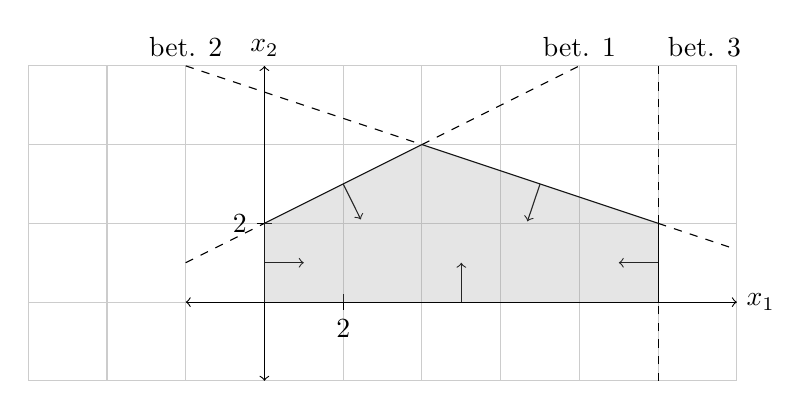
\begin{tikzpicture}
  %laver Grid. godt til når koordinater skal redigeres
  	\draw[thin,gray!40] (-3,-1) grid (6,3); 
  %x-aksen
  	\draw[<->] (-1,0)--(6,0) node[right]{$x_1$};
  	\draw[->] (2.5,0) -- (2.5,0.5);
  %y-aksen
  	\draw[<->] (0,-1)--(0,3) node[above]{$x_2$};
  	\draw[->] (0,0.5) -- (0.5,0.5);
  	
  %akse-markeringer
  	%\node[left] (xakse) at (0,1) {2};
  	\draw[] (-0.1,1) -- (0.1,1) node[pos=0,left] {2};
  	\draw[] (1,-0.1) -- (1,0.1) node[pos=0,below] {2};
  	
  %ligning 1
	\draw[domain=-1:0,variable=\x,dashed] 	plot({\x},{0.5*\x+1});
	\draw[domain=0:2,variable=\x] 			plot({\x},{0.5*\x+1});
	\draw[domain=2:4,variable=\x,dashed] 	plot({\x},{0.5*\x+1}) node[above] {bet. 1};
  	\draw[->] (1,1.5) -- (1.224,1.05);
	
  %ligning 2
  	\draw[domain=-1:2,variable=\x,dashed] 	plot({\x},{-(1/3)*\x+8/3}) node[above] at (-1,3) {bet. 2} ;
	\draw[domain=2:5,variable=\x] 			plot({\x},{-(1/3)*\x+8/3});
	\draw[domain=5:6,variable=\x,dashed] 	plot({\x},{-(1/3)*\x+8/3});
	\draw[->] (3.5,1.5) -- (3.34,1.026);

  %ligning 3
  	\draw[domain=-1:0,variable=\y,dashed] 	plot({5},{\y});
	\draw[domain=0:1,variable=\y] 			plot({5},{\y});
	\draw[domain=1:3,variable=\y,dashed] 	plot({5},{\y}) node[above right] {bet. 3};
	\draw[->] (5,0.5) -- (4.5,0.5);

  %løsningsmængden skraveret
	\fill[gray!80,nearly transparent] (0,0) -- (0,1) -- (2,2) -- (5,1) --(5,0) --  cycle;
\end{tikzpicture}
%	\captionof{figure}{Den mulige mængde af et standard maksimeringsproblem.}
%	\label{fig:maksprob2}
%\end{center}

\label{eks:maksprob2}
\end{eks}

%%%%%%%%%%%%%%%%%%%%%%%%%%%%%%%%%%%%%%%%%%%%%%%%%%%%%%%%%%%%%%%%%%%%%%%%%%%%%%%%%%%%%%%%%%%%%%
%%%%%%%%%%%%%%%%%%%%%%%%%%%%%%%%%%%%%%%%%%%%%%%%%%%%%%%%%%%%%%%%%%%%%%%%%%%%%%%%%%%%%%%%%%%%
Da bibetingelserne er ligninger repræsenteret ved et prikprodukt, kan hele ligningssystemet repræsenteres som et matrix-vektorprodukt, det kræver dog, at alle ikke positivitets betingelser er på samme form.
Det kan derfor være favorabelt at kunne omskrive fra en ulighed til en anden.
\begin{stn}
Lad $\vec{a}_i^T,\vec{x} \in \mathds{R}^n$ og $b_i \in \mathds{R}$, da gælder:
\begin{enumerate}
\item $\vec{a}_i^T\vec{x} \geq b_i \quad \Leftrightarrow \quad -\vec{a}_i^T\vec{x} \leq -b_i$
\item $\vec{a}_i^T\vec{x} = b_i \quad \Leftrightarrow  \quad  \vec{a}_i^T\vec{x} \leq b_i \quad \wedge \quad  \vec{a}_i^T\vec{x} \geq b_i$
\item $\vec{a}_i^T \vec{x}  \leq b_i \quad \Rightarrow \quad  \vec{a}_i^T \vec{x}  +  x_{n+i}  = b_i$
\item $\vec{a}_i^T \vec{x}  \geq b_i \quad \Rightarrow \quad  \vec{a}_i^T \vec{x}  - x_{n+i}  = b_i$
\end{enumerate}
hvor $x_{n+i}$ er en slack variable. 
\end{stn}
Dermed kan bibetingelserne skrives som $A\vec{x}\geq \vec{b}$, hvor $\vec{a_i}$ udgør den $i$te række i $A$ og $b_i$ er den $i$ indgang i $\vec{b}$.
Bemærk at positivitetsbetingelserne er et særtilfælde af størreendbetingelser, hvor en koefficienten til $x_i$ er 1, mens resten af koefficienterne er 0 og hvor $b_i=0$.
Positivitets betingelsen skrives ikke med i ligningssystemet, og i stedet er det som oftes underforstået, at enhver variable skal være ikke negativ.
For at det skal gøre sig gældende, skal en hver frivariable omskrives så de er betinget af en positivitetsbetingelse.
\begin{stn}
Lad $x_i$ være en frivariabel, da er $x_i = x_{n+i}-x_{n+i+1}$, hvor $x_{n+i},x_{n+i+1}\geq 0$.
\end{stn}